\documentclass{wileySix}
\usepackage{w-bookps}

% \usepackage{mathptmx}

\usepackage{graphicx}
\usepackage{enumitem}

\setcounter{secnumdepth}{3}

\setcounter{tocdepth}{2}

\begin{document}

\booktitle{Web Service}
\subtitle{Semua Tentang Komunikasi antar Aplikasi Berbasis Protokol internet}

\author{Rolly Maulana Awangga}

\halftitlepage
\titlepage



\offprintinfo{Web Service, pre-release}{Rolly Maulana Awangga}


\begin{copyrightpage}{2018}
Web Service / Rolly Maulana Awangga
\end{copyrightpage}


\dedication{For my family}

\contentsinbrief %optional
\tableofcontents
\listoffigures %optional
\listoftables  %optional

%%%%%%%%%
%%Content 
%%%%%%%%%

\part[Pengenalan Web Service]
{Pengenalan\\ Web Service}

\chapter[Contoh]
{Contoh\\ Latex}
tugas 1 :
Tuliskan resume atau tutorial;

2A :
1. Python instalasi dan definisi dan contoh kode awal
2. wsgi definisi dan contoh contoh
3. cgi definisi dan contoh
4. uwsgi instalasi definisi dan contoh
5. Install the Windows Subsystem for Linux


2B :
1. contoh aplikasi web service
2. pengertian web service
3. protokol
4. port
5. penggunaan aplikasi testing web service


2C :
1. internet
2. web
3. backend
4. frontend

Syarat :
1. gunakan SPOK yang benar
2. Tanda baca yang benar
3. Penggunaan Huruf kapital yang benar

buat grup kelompok di github dan fork webservice

Parameter(baca standar penulisan latex) :
1. itemize dan enumerate yang benar (10)
2. gambar dan referensi disebutkan dalam kalimat dengan benar (10)
3. penggunaan section subsection subsubsection yang benar (10)
4. Penggunaan tabel atau verbatim atau equation (10)
5. commit sehari(min 50 kata) per anggota kelompok selama 6 hari (60)

Nilai akhir X persentasi plagiarisme = Nilai tugas

(GUnakan standar penggunaan git)
jika ada error maka minus 5 setiap kali pull request

\chapter[RESTful]
{Definisi\\ RESTful}
\begin{itemize}
\item Ahmad Syafrizal Huda (1164062)
\item Annisa Fathoroni (1164067)
\item Puad Hamdani (1164084)
\item Rahmi Roza (1164085)
\item Tasya Wiendhyra (1164086)
\end{itemize}

\section{Definisi RESTful Web Service}
REST merupakan salah satu macam web service yang memasukkan konsep perpindahan antar state. State disini bisa dibayangkan seperti jika browser meminta suatu halaman web, maka server akan mengirimkan state halaman web yang sekarang ke browser. Menurut salah satu perkembangan Tidwell, D., 2001 bernavigasi melalui link-link yang disediakan sama halnya dengan mengganti state dari halaman web. Begitu pula REST bekerja, dengan bernavigasi melalui link-link HTTP untuk melakukan aktivitas tertentu, seakan-akan terjadi perpindahan state satu sama lain \cite{indrawan2017implementasi}.
Pada gambar \ref{labelgambar} menerangkan cara Rest Web Service melakukan request kepada server kemudian server membalasnya dengan result berupa json. Metode tersebut telah dikembangkan oleh Roy Thomas Fielding dalam disertasinya tentang Architectural Style.  Dalam disertasinya tersebut REST (Representational state transfer) didefinisikan sebagai suatu gaya arsitektur perangkat lunak untuk pendistribusian sistem hypermedia seperti WWW \cite{rofiq2017implementasi}.
\begin{figure}[ht]
\centerline{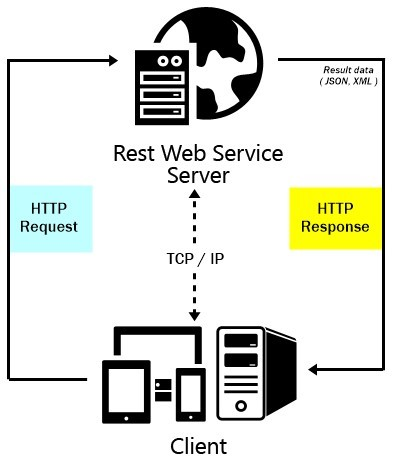
\includegraphics[width=1\textwidth]{figures/1restful.JPG}}
\caption{RESTful}
\label{labelgambar}
\end{figure}

\section{Prinsip atau Karakter Pada RESTful}
RESTful adalah salah satu teknologi web service untuk membuat suatu sistem yang terdistribusi dimana cara kerjanya berdasarkan resource. RESTful sendiri merupakan software yang didesain untuk penekanan pada skalabilitas,kesederhanaan dan kegunaan. Metode dalam REST terdiri dari empat prinsip utama teknologi, yaitu \cite{aji2016penerapan}:
\begin{enumerate}
\item Resource identifier melalui Uniform Resource Identifier (URI), REST Web service mencari sekumpulan sumber daya yang mengidentifikasi interaksi antar klien.
\item Uniform interface, sumber daya yang dimanipulasi CRUD (Create, Read, Update, Delete) menggunakan operasi PUT, GET, POST, dan DELETE.
\item Self-descriptive messages, sumberdaya informasi tidak terikat, sehingga dapat mengakses berbagai format konten (HTML, XML, PDF, JPEG, Plain Text dan lainnya). Metadata pun dapat digunakan.
\item Stateful interactions melalui hyperlinks, setiap interaksi dengan suatu sumber daya bersifat stateless, yaitu request messages tergantung jenis kontennya.
\end{enumerate}

\section{Sejarah RESTful}
REST tidak menarik perhatian banyak ketika pertama kali diperkenalkan pada tahun 2000 oleh Roy Fielding di Universitas California, Irvine, dalam disertasinya akademik, Architectural gaya dan arsitektur perangkat lunak berbasis desain jaringan, yang menganalisa set dari prinsip-prinsip arsitektur perangkat lunak yang menggunakan Web sebagai platform untuk komputasi terdistribusi (Lihat sumber daya untuk link ke disertasi ini). Sekarang, tahun setelah diperkenalkan, utama kerangka untuk REST telah mulai muncul dan masih sedang dikembangkan karena itu dijadwalkan, misalnya, akan menjadi bagian integral dari Java 6 melalui JSR-311 \cite{rodriguez2008restful}.

\section{Contoh-Contoh Penerapan  RESTful}
\subsection{Implementasi RESTful Web Service untuk Sistem Penghitungan Suara Secara Cepat pada Pilkada}
Metode ini yang digunakan oleh penyelenggara pemilihan umum untuk menentukan hasil pilkada. Dengan memanfaatkan teknologi yang ada, proses pengumpulan data hasil perolehan suara bisa dilakukan dengan lebih cepat. Salah satu metode baru yang bisa digunakan untuk melakukan proses tersebut adalah metode perhitungan cepat riil. Metode ini memanfaatkan teknologi informasi dan komunikasi untuk melakukan proses penghitungan suara. Real-quick count mengambil hasil perhitungan dari semua tempat pemungutan suara (TPS). Tetapi hasil tersebut dikirim langsung dari TPS ke lembaga penyedia informasi hasil perhitungan cepat, tidak melalui prosedur seperti pada real count yang mengharuskan pengumpulan data berjenjang, oleh karena itu waktu yang dibutuhkan untuk memperoleh semua hasil suara bisa dioptimalkan. Pada jurnal ini dilakukan perbandingan antara SOAP dan REST pada aplikasi mobile dan multimedia conference. Hasil penelitian yang dilakukan pada aplikasi mobile computing menunjukkan bahwa ukuran pesan pada RESTful web service mencapai 9 sampai 10 kali lebih kecil dibandingkan ukuran pesan dari web service berbasis SOAP \cite{rofiq2017implementasi}.

\subsection{Implementasi RESTful untuk Sales Order dan Sales Tracking Berbasis Mobile}
Bagian penjualan merupakan bagian yang paling penting dalam penjualan produk. Perusahaan membutuhkan sistem yang dapat membantu aktivitas dan pemesanan produk. dengan membuat sebuah Controller terlebih dahulu,yang berperan untuk menentukan informasi apa yang akan disampaikan pada saat client mengakses web service. Dibuat dengan arsitektur REST dengan menggunakan method yang di dukung protokol HTTP seperi method DELETE, UPDATE, CREATE,dll. Aplikasi mobile ini akan menggunakan data dari GPS untuk memastikan lokasi penjual juga dilengkapi barcode untuk mempercepat input data barang \cite{kurniawan2015implementasi}.

\subsection{Implementasi REST Web Service Pada Aplikasi Pengolah Pesan Yahoo Messenger Pada CV. Meliana Pratama}
Mengimplementasikan REST Web Service pada aplikasi pengolah pesan Yahoo Messenger (YM). Aplikasi REST Web Service dapat dijadikan sebagai miidleware antara aplikasi pengolahan pesan Yahoo Messenger (YM) dengan database, sehingga proses transaksi ke database menjadil lebih efisien. Hal ini dikarenakan aplikasi client tidak perlu mengetahui database apa yang digunakan oleh server \cite{ikrom2015implementasi}.

\subsection{Implementasi RESTful Web Service Pada Aplikasi Iklan Baris Online}
Pada implementasi aplikasi ini menerapkan restful web service yang dimana server akan berinteraksi dengan client pada interface yang sama atau seragam. Server akan meng-host resource sedangakn client akan menjadi konsumen dari resource yang disediakan server. Pada saat server meminta atau request data script request akan dikirim dari client ke server berbentuk alamat url yang kemudian memanggil file PHP yang mengakses data dari databse server. saat pengambilan data, client akan memanfaatkan API yang terdapat dalam server. Setelah mendapat data dari client, server kemudian akan menyebar informasi yang dibutuhkan berupa kebutuhan barang/jasa yang bersangkutan kepada member atau client \cite{fauziah2014aplikasi}.

\subsection{Implementasi Protokol OAuth 1.0 Sebagai Autentikasi pada Aplikasi SMS Blast Berbasis Android}
Sebuah aplikasi SMS Blast berbasis Android dan sebuah web service yang digunakan oleh aplikasi untuk melakukan request terhadap data nomor telepon terhadap data yang sudah ada. OAuth menggunakan token pada setiap request. Web service akan membangkitkan token yang berbeda pada setiap request dari consumer. Penggunaan token ini dapat meminimalkan kemungkinan terjadinya serangan Man in the Middle Attack dan Hijacking Attack
\cite{saputra2017implementasi}

\subsection{Implementasi RESTful Web Service One Chip Multi-Client Untuk Mengoptimalkan Penjualan Pulsa All Operator}
One  Chip  All  Operator adalah sebuah chip untuk pengisian pulsa kesemua operator selluler GSM dan CDMA bahkan juga dapat digunakan untuk pengisian pulsa listrik atau listrik prabayar. Chip atau kartu perdana  yang  digunakan bukan kartu Khusus atau tidak harus dipesan kedealer penyedia pelayanan pengisian pulsa,Chip yang   digunakan cukup perdana biasa,jadi nomor  yang dipakai sehari-hari dapat dijadikan sebagai chip untuk pengIsian pulsa ke semua operator. Proses awal yang dilakuakanya itu peses deployment restful  web  service. Deployment  restful web service  merupakan proses menjalankan web service pada server seperti apache tomcat agar aplikasi client dapat mengakses service database\cite{indrawan2017implementasi}.

\subsection{Implementasi Protocol Buffers pada Aplikasi Weblog Client dan Server}
Web service yang digunakan untuk mengirimkan dan menerima   protobuf  messages adalah  RESTful  web service  yang  merupakan  teknologi  web  service  yang ringan dan mudah diimplementasikan. Client mengirimkan data yang telah diserialisasikan dalam bentuk protobuf message melalui  HTTP  request kepada RESTful  service pada server. Protobuf  message kemudian diubah menjadi data semula dengan program deserialisasi yang telah ada di server \cite{wibowo2011implementasi}.

\subsection{Implementasi Restful Web Service Menggunakan AsyncTask pada Aplikasi Library Automation Berbasis Android}
Dengan menggunakan aplikasi Library automation berbasis android ini diharapkan dapat mempermudah untuk mengakses informasi terkait referensi yang terdapat pada perpustakaan fisik penggunaan RESTful web service dengam menggunakan AsyncTask sebagai prosesnya juga dinilai cukup baik dari segi penggunaan. Diharapkan untuk pengembangan selanjutnya meningkatkan akurasi pencarian supaya end user tidak merasa bingung saat mencari informasi \cite{yudhistiraimplementasi}.

\subsection{Penerepan Restful pada Aplikasi Ayo Piknik Indonesis Berbasis Android}
Aplikasi Ayo Piknik Indonesia berbasis android yang berbasis dengan Web-server menggunakan metode Restful Webservice yang bisa menampilkan informasi wisata dengan cepat dan tepat serta pengguna juga dapat memberikan usulan tempat wisata yang baru. Kemudian akan dilakukan verifikasi agar bisa ditampilkan. Selain itu aplikasi ini juga  dapat menambahkan data wisata dengan google maps untuk memudahkan wisatawan ataupun penduduk lokal \cite{aji2016penerapan}.

\section{Pengembangan Sistem Informasi RESTful Web Service}
Pengembangan sistem informasi kependudukan berbasis mobile dan restful pada web service yaitu\cite{kurniawati2016pengembangan}:
\begin{enumerate}
\item REST Web Service pada tahap ini akan dibuat web service yang diletakkan pada server pusat untuk mengolah data JSON. Web service memiliki 3 method yaitu json decode yaitu untuk parsing data masukan, StoreData dan json encode parsing untuk data keluaran. Parameter masukan dari database SQLite ke MySQL tampak pada gambar 5, akan diparsing ke dalam format Array. StoreData yang berhubungan langsung dengan database dalam proses input, status gagal atau sukses akan disimpan dalam Array dan diolah lagi menjadi format JSON sebagai keluaran dari web service.
\item Aplikasi Android Antarmuka aplikasi android saat dijalankan akan muncul form login. Pengguna aplikasi yaitu kepala lingkungan memasukkan username dan password kemudian tekan tombol login
\end{enumerate}

\subsection{Pengembangan Sistem Informasi Kependudukan Berbasis Moblie Dan RESTFful Web Service}
Sensus biasa dilakukan secara manual, yaitu door-to-door ke setiap rumah warga namun hal tersebut membutuhkan waktu yang lama dan tidak cukup efektif, lalu dibuat solusi dari permasalahan tersebut dengan mengintegrasikan RESTful web service pada perangkat Android. Diimplementasikan pada Android karena Android memiliki kelebihan dapat mengakses database secara offline yaitu SQLite sehingga lokasi yang berada di pedalaman tetap dapat terinputkan ke database meski tidak ada jaringan internet.
Cara kerjanya yaitu petugas sensus akan memasukan data di perangkat android, yang kemudian datanya akan dimasukkan kedalam database. Webservice RESTful ini berfungsi sebagai komunikator antara android dengan database pusat. Web service ini diletakkan di server pusat untuk mengolah data JSON. Parameter masukkan dari SQLite ke MySQL akan di parsing ke format array yang diubah lagi menjadi JSON sebagai hasil dari web servicenya \cite{kurniawati2016pengembangan}.

\section{Kelebihan dan Kekurangan RESTful Web Service}
Pada tabel \ref{table:contoh} merupakan kelebihan dan kekurangan daripada RESTful Web Service dimana RESTful Web Service ini sangat berguna dalam implementasinya \cite{nugroho2012perbandingan}.
\begin{table}[h]
\begin{tabular}{|c|c|c|}
\hline
Jenis Web Service&Kelebihan&Kekurangan\\
\hline
RESTful Webs Service&-Implementasi RESTful Web Service relatif& -Struktur data yang sangat kompleks\\
&sederhana dalam hal pemrogramannya karena& sukar diadaptasi ke dalam URL.\\
&menggunakan standar-standar yang telah&\\
&diterima secara luas (HTTP, XML, dan URL).&\\
&-Server dan klien HTTP dikenali&-Implementasi dan kinerjanya sangat bergantung\\
&oleh sebagian besar bahasa pemrograman&pada kapasitas jaringan yang digunakan\\
&dan hampir semua platform perangkat&\\
&keras/perangkat lunak yang saat ini populer.&\\
\hline
\end{tabular}
\label{table:contoh}
\end{table}

\section{Implementasi PHP Web Service Sebagai Penyedia Data Aplikasi Mobile}
Dapat disimpulkan bahwa PHP Web Service bisa diimplementasikan dalam aplikasi mobile yang membutuhkan data dinamis. Pengujian atas web service bisa dilakukan dengan membuat file PHP secara manual ataupun menggunakan SOAP web service. Untuk memudahkan pemanggilan data bisa dilakukan modifikasi dengan memberikan layer tambahan berupa PHP File yang memanggil pada SOAP web service
\cite{surendra2014implementasi}.


%\chapter[Web]
%{Definisi\\ Web}
%%\begin{itemize}
%\item Imron Sumadireja (1164076)
%\item Jesron Marudut (1164077)
%\item Lusia Violita Aprilian (1164080)
%\item Mhd. Zulfikar Akram Nst. (1164081)
%\end{itemize}

\section{Pengertian Website}
World wide web (www atau web) merupakan halaman situs informasi yang dapat diakses secara cepat atau sarana
antar muka informasi di internet. Web dapat menggabungkan teks, grafik, dan multimedia. Web memudahkan
penggunanya untuk mengakses informasi melalui konsep hypertext sehingga memungkinkan  suatu text untuk
menjadi acuan membuka dokumen laindo. Informasi dapat mudah disebar dan diakses.

\subsection{Sejarah Website}
Sementara itu World wide web (www) dikembangkan pertama kali oleh Tim Berners-Lee pada tahun 1989. Pada
awalnya, Tim mengusulkan WWW sebagai suatu cara berbagai dokumen diantara para peneliti. Dokumen online dapat
diakses melalui alamat unik yang disebut Universal Resource Locator atau URL. Selain itu WWW tidak hanya
dikembangkan untuk keperluan para peneliti, namun juga dikembangkan untuk kalangan pendidikan, bisnis dan
perorangan. Berdasarkan penjelasan singkat diatas dapat disimpulkan bahwa antara web dan internet memiliki
hubungan yang sangat erat walaupun keduangnay tidak bisa dikatakan sama. Web merupakan bagian dari layanan
yang dapat berjala di atas teknologi internet.

\subsection{Jenis-jenis website}
Website dikelompokan dalam beberapa jenis-jenis Website agar dapat memudahkan dalam menentukan jenis website
yang akan ditentukan. Dan berikut jenis-jenis website yang dikelompokan atas beberapa dasar:
\begin{enumerate}
\item Jenis Website berdasarkan sifat;
\begin{itemize}
\item Website Statis, merupakan web yang kontenya hampir jarang diubah
\item Website Dinamis, Web yang konten atau isinya dapat berubah-ubah setiap saat
\end{itemize}
\item Jenis Website yang dikelompokkan berdasarkan Bahasa Pemrogramannya;
\begin{itemize}
\item Server side, Website yang memakai bahasa pemrograman yang tergantung dengan servernya
\item Client side, adalah web yang tidak perluu server untuk menjalankannya. Cukup diakses dengan browser.
\end{itemize}
\item Jenis-jenis Web menurut tujuannya;
\begin{itemize}
\item Web personal, biasanya web ini merupakan web yang berisi informasi seorang
\item Corporate Web, website yang dimiliki sebuah institusi atau perusahaan.
\item Web Portal, Web ini berisi banyak layanan, seperti berita, email dan jasa
\item Web Forum, sebuah web yang dibuat sebagai sarana diskusi.
\end{itemize}
\end{enumerate}
	
\subsection{Keuntungan Web}
Keuntungan penggunaan web diantaranya yaitu :
\begin{itemize}
\item Informasi dapat diberikan segera(tepat waktu) dan diperbarui secara berkala.
\item Presentasi fleksible dan visibilitas dapat menyediakan ragam isyarat untuk diseminasi informasi.
\item Informasi dapat diorganisir melalui tautan dan menu, berbagai tingkatan informasi dapat disediakan format file yang berbeda dapat digunakan untukj informasi yang dapat diunduh. Integrasi informasi dapat dilakukann melalui tautan dan seksi lain, halaman lain, atau web lain.
\item Tauta  dan menu dapat menyediakan informasi bagi pemangku kepentingan yang berbeda, informasi dapat pula diberikan melalui daftar email kepada pemangku kepentingan.
\item Setiap orang yang dapat mengakses web dapat memperoleh informasi karena keterjangkauan global dan potensi komunikasi masl dari web.
\end{itemize}
	   
\section{tentang web scraping}
Web scraping atau scraping web (dapat disebut juga panen web atau web ekstraksi data) merupakan sebuah
perangkat lunak komputer teknik penggalian informasi dari situs web seperti mengambil mengambil data
berbentuk teks yang umumnya bertipe HTML atau XHTML. contohnya seperti Internet Explorer (IE) dan Mozilla Web
Browser. web scraping berkaitan erat dengan pengindekan web.

\subsection{manfaat dari web scraping}
Web scraping sering dikenal dengan screen scraping. Web scraping tidak dapat dimasukkan kedalam bidang data
mining karena dalam data mining menyiratkan upaya untuk memahami pola semantik dari sejumlah data besar yang
telah diperoleh. Aplikasi Web scraping hanya fokus pada cara memperoleh data melalui pengambilan dan ekstrasi
dengan ukuran data yang bervariasi. Manfaat dari web scraping adalah agar informasi yang diambil lebih
terfokus sehingga dapat memudahkan dalam melakukan pencarian sesuatu, adapun cara untuk mengembangkan teknik
web scraping yaitu dengan cara sebagai berikut:
\begin{enumerate}
\item Pengembang/pembuat program mempelajari dokumen HTML dari website yang akan diambil informasinya untuk
di tag HTML tujuannya yakni untuk mengapit informasi yang akan diambil (Create Scraping Template)
\item Pengembang/pembuat program mempelajari teknik navigasi pada website yang akan diambil informasinya
untuk ditiru pada aplikasi web scraping yang akan dibuat (Explore Site Navigation)
\item Selanjutnya aplikasi web scraping akan mengotomisasi informasi yang didapatkan dari website yang telah
ditentukan (Automate Navigation and Extraction), informasi yang didapat tersebut akan disimpan dalam 
tabel basis data (Extracted Data and Package History).
\end{enumerate}

\subsection{Perbandingan Metode Web Scraping}
Berikut perbandingan antara metode Web Scraping menggunakan CSS Selector dan Xpath Selector
\begin{enumerate}
\item Penggunaan metode XPATH Selector untuk web scraping menghasilkan artikel yang lebih lengkap
dibandingkan dengan menggunakan metode CSS Selector, Ditunjukkan dengan jumlah item dan ukuran file
yang didapatkan lebih besar. Namun juga menyisakan proses lain untuk menghilangkan kode HTML yang tidak
diinginkan dari artikel yang dihasilkan menggunakan metode XPATH Selector.
\item Dalam penggunaan memori baik metode XPATH Selector dan CSS Selector tidak memiliki perbedaan yang
signifikan(cenderung sama). Disebabkan karena engine scrapy yang baik dalam penggunaan resource-nya. 
\item Metode XPATH Selector memiliki waktu proses yang lebih cepat daripada menggunakan metode CSS Selector.
\item Pada metode XPATH, selector cukup mengikuti node pada halaman web, sehingga waktu yang dibutuhkan
relatif lebih singkat.
\end{enumerate}

\section{Tentang Web Hosting}
Web hosting merupakan jasa penyewaaan tempat penyimpanan data di internet atau biasa disebut dengan cloud
yang diperlukan oleh sebuah website. Web hosting ialah salah satu syarat agar website bisa diakses secara 
online dan dapat diakses dari seluruh dunia. Ukuran yang digunakan dalam suatu web hosting adalah kapasitas
dan bandwidth. Kapasistas merupakan ukuran besarnya kemampuan sebuah web hosting untuk menyimpan data-data di internet.

Bandwidth merupakan ukuran maksimal dari jumlah volume data yang diperbolehkan untuk diakses dari web hosting
setiap bulannya. Sebagai contoh, sebuah halaman website yang mempunyai ukuran 2 MB dan bandwidth web hosting
2000 MB, maka setiap bulannya website tersebut dapat diakses sebanyak 2000 kali.

\subsection{Tentang Domain}
Domain merupakan sebuah alamat di dunia internet atau sebuah identitas dari sebuah website. Domain digunakan untuk mempermudah dalam mengakses situs yang ada di internet. Domain terbagi menjadi 2 jenis domain yang dibagi berdasarkan pemisahaan titiknya, yaitu; Top Level Domain (TLD) dan Second Level Domain (SLD). Top Level Domain merupakan bagian terakhir dalam sebuah domain website. Contohnya "facebook.com" dan disitu yang jadi domainnya adalah ".com". Selanjutnya Second Level Domain atau SLD merupakan bagian dari domain yang terdapat sebelum Top Level Domain. Contohnya "Facebook.com" yang menjadi SLDnya adalah Facebook. Jadi SLD adalah unsur domain yang didaftarkan terdahulu pada jasa Web Hosting. Dan ada juga yang disebut Country Code Second Level Domain (ccSLD). Berguna sebagai penunjuk organisasi apa yang mendaftar pada suatu domain. Setiap negara juga mempunyai ccSLD yang berbeda-beda tiap negaranya.

\subsection{Tentang Hubungan Domain dan Web Hosting}
Hubungan Domain dan Web Hosting merupakan satu kesatuan yang saling membutuhkan. Pada sebuah Website, domain dan web hosting saling ketergantungan. Apabila yang tersedia hanya web hosting, maka website tidak akan dapat diakses. Begitu juga dengan domain, apabila yang tersedia hanya domain, maka tidak akan ada website yang akan ditampilkan, karena halaman website tersimpan didalam web hosting.

\subsection{Macam-macam Web Hosting}
Saat ini banyak jasa penyedia hosting dengan harga relatif murah bahkan gratis. Berikut adalah macam-macam web hosting :
\begin{enumerate}
\item Free Hosting / Web Hosting Gratis
Dengan free hosting, kita dengan mudah mencari layanan web hosting dan domain gratis di internet dengan menggunakan fasilitas search engine seperti google atau yang lainnya. Biasanya penyedia web hosting tidak mengenakan biaya. Namun, memiliki banyak keterbatasan beberapa fitur.
\item Web Hosting Berbagi atau Shared Hosting
Jenis hosting ini paling sering digunakan karena bukan hanya murah, namun juga memiliki layanan yang  dapat mencukupi segala kebutuhan. Biasanya, untuk menggunakan layanan web hosting ini anda hanya perlu untuk mengeluarkan biaya sebesar 100 hingga 200 ribu untuk mendapatkan ruang sebesar 2 GB – 7,5 GB dengan bandwith unlimited.
\item VPS Web Hosting
VPS merupakan singkatan dari Virtual Private Server. Jadi disini anda dapat seperti memiliki server sendiri untuk situs anda. dengan server ini, anda akan memiliki control yang lebih dalam seperti Dedicated Server.
\item Dedicated Web Hosting
Dedicated Web Hosting merupakan sebuah layanan hosting dengan server yang memiliki kemampuan untuk melakukan handle terhadap traffic dengan jumlah sangat banyak. Serta memiliki banyak fitur premium di dalamnya. Selain itu,juga memiliki control penuh terhadap server walaupun  hanya menyewanya.
\item Managed Web Hosting
Managed Hosting / Web Hosting Terkelola ini adalah web hosting yang dikhususkan untuk situs dengan. Platform yang sama. Managed web hosting biasanya lebih aman dan kinerjanya lebih optimal. Selain itu, memudahkan untuk melakukan beragam pengaturan, mulai dari installasi, sampai setting macam-macamnya.
  \end{enumerate}

\subsection{Cara Mendapatkan Web Hosting dan Domain}
Web hosting dan domain lebih sering ditemukan oleh perusahaan-perusahaan penyedia web hosting atau domain. Untuk menemukannya, cukup cari di google. Maka akan banyak perusahaan yang menyediakan jasa web hosting. Kinerja web hosting berbeda-beda dari setiap perusahaan Web hosting. Karna apabila web hosting yang dibuat oleh jasa tersebut buruk maka website tersebut akan mudah bermasalah. Oleh karena itu dalam pembelian jasa domain atau web hosting perlu diperhatikan hal-hal seperti profil dari penjual web hosting, fitur untuk website dan harga dari web hosting tersebut. Dalam memilih penyedia web hosting, pastikan penyedia mempunyai reputasi yang bagus dan terpercaya. Dan sebaiknya memilih perusahaan web hosting yang sudah dalam bentuk perusahaan CV atau PT agar pertanggung jawabannya jelas ketika terjadi gangguan web hosting.
	
\section{Apa itu cPanel?}
Apa itu cPanel?
cPanel adalah perangkat lunak control panel online untuk melakukan pengaturan website dalam sebuah web histing. cPanel adalah tool utama untuk pengguna web hosting. 
Beberapa fungsi utama cPanel antara lain yaitu upload data website, pengaturan data website, instalasi content management system, dan lain-lain. Melelui cPanel juga kita bisa mengatur data-data website. Kita bisa menambah, menghapus, atau memodifikasi data website.

\subsection{Backup date dengan cPanel}
Kemudahan yang diberikan cPanel sebagai control panel yakni untuk mempermudah proses hosting di suatu situs web menggunakan 3 tingkatan struktur untuk memberikan fungsi administrator, agen, dan yang memiliki situs web tersebut untuk mengatur berbagai macam aspek dari situs web dan administrasi server melalui sebuah web standar. Dalam menu cPanel untuk backup disediakan 3 pilihan layanan backup yang ada yakni:
\begin{enumerate}
\item System Backup, merupakan menu backup yang dapat digunakan untuk mendownload backup otomatis yang telah dibuat oleh administrator server
\item Full Backup, akan melakukan backup file untuk mengembalikan file yang corrupt, terhapus atau pindah pada server yang lain.
\item Backup Home Directory, berfungsi untuk memberikan hak akses untuk mengambil file yang berada pada directory home.
\end{enumerate}


%\chapter[Backend]
%{Definisi\\ Backend}
%\input{section/1Backend.tex}

%\chapter[Frontend]
%{Frontend}
%\input{section/1Frontend.tex}

% contoh aplikasi web service
% web service
% protokol
% port

% HTTP
% URL
% POST
% GET


\bibliographystyle{IEEEtran}.
\bibliography{references}.

\printindex

\end{document}
